\documentclass{article}
\usepackage{graphicx} % Required for inserting images

\title{DevOps24-groupK\\
\large Course Code: BSDSESM1KU}
\author{GitGurus}
\date{Spring 2024}

% \usepackage{graphicx} % Required for inserting images
% \usepackage{amsmath}
% \usepackage{hyperref}
\usepackage{listings}
\lstset
{
    basicstyle=\footnotesize,
    numbers=left,
    stepnumber=1,
    showstringspaces=false,
    tabsize=1,
    breaklines=true,
    breakatwhitespace=false,
}

\usepackage[utf8]{inputenc}
\usepackage[T1]{fontenc}
\usepackage[english]{babel}
\usepackage{minted}
% \usepackage[a4paper, bottom=3cm, top=3cm, left=2.5cm, right=2.5cm]{geometry}
\usepackage[linewidth=1pt]{mdframed}
\usepackage{ebproof}
\usepackage{amsmath}
% \usepackage{fourier}
\usepackage{booktabs}
% \usepackage{inconsolata}
\usepackage{float}
\usepackage{lastpage}
\usepackage{graphicx}
\usepackage{titling}
\usepackage{fancyhdr}
\usepackage[dvipsnames]{xcolor}
\usepackage[hidelinks]{hyperref}

\renewcommand{\baselinestretch}{1.2} % Line spacing
% \setlength{\parindent}{0em} % Paragraph indent
% \setlength{\parskip}{0.75em} % Paragraph vertical spacing

% \colorlet{LightGray}{Gray!7!}

% % global minted styles
% \setminted{bgcolor=LightGray, breaklines, frame=single, linenos, fontsize=\small, numbersep=8pt}

% % minted remove red squares around "erroneus" code
% \AtBeginEnvironment{minted}{%
%   \renewcommand{\fcolorbox}[4][]{#4}}

% % minted line number style
% \renewcommand{\theFancyVerbLine}{{\scriptsize \arabic{FancyVerbLine}}}
\begin{document}

\maketitle

\begin{table}[H]
    \centering
    \begin{tabular}{c|c}
    Andreas Guldborg Hansen & aguh@itu \\
    Andreas Severin Hauch Trøstrup & atro@itu.dk \\
    Frederik Petersen & frepe@itu.dk \\
    Mads Aqqalu Roager & mroa@itu.dk \\
    Silke Holme Bonnen & ssbo@itu.dk
    \end{tabular}
\end{table}

\newpage
\tableofcontents

\newpage


\section{Systems' perspective}
\subsection{Design and architecture}
\begin{figure}[H]
    \centering
    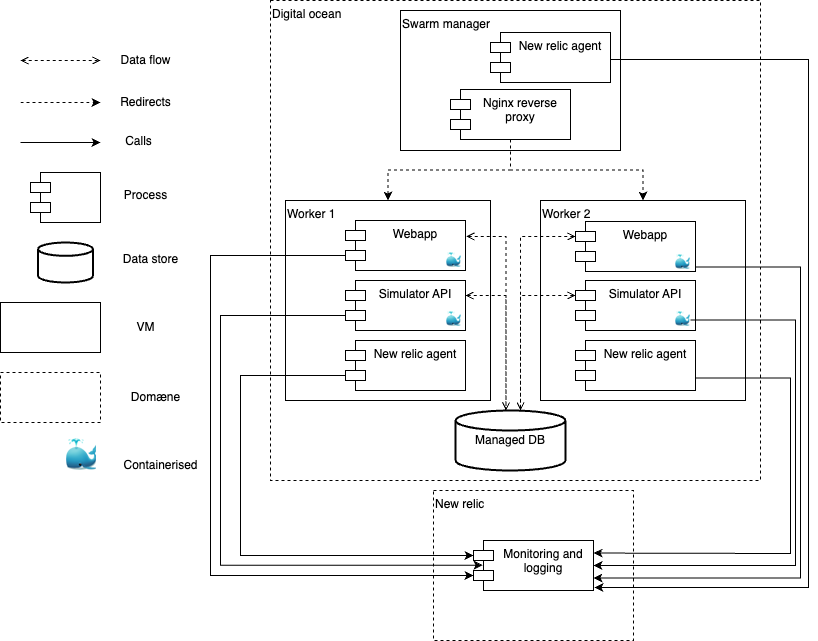
\includegraphics[width=\textwidth]{images/devops-overview.png}
    \caption{A diagram of the infrastructure running our application}
    \label{fig:infrastructure}
\end{figure}

\subsection{Dependencies}

\subsection{Interactions of subsystems}

\begin{figure}[H]
    \centering
    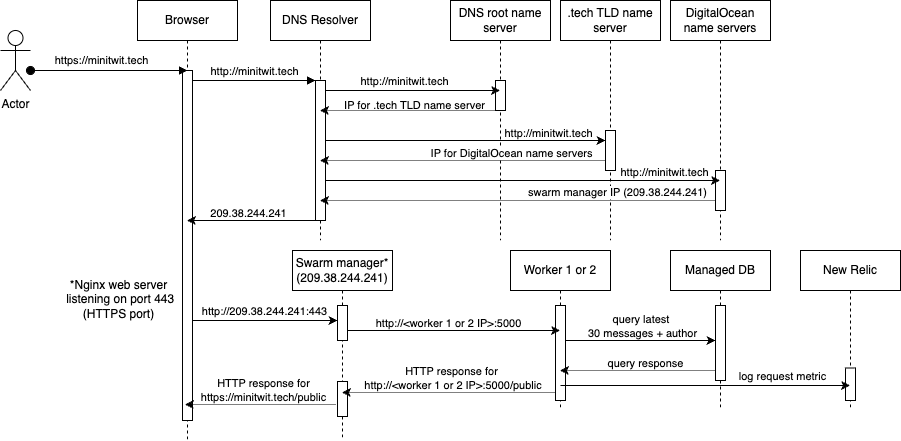
\includegraphics[width=\textwidth]{images/devops-sequence.png}
    \caption{A sequence diagram describing the process of calling "minitwit.tech/public"}
    \label{fig:sequence}
\end{figure}

\subsection{Current state}

\section{Process' perspective}

\subsection{CI/CD chain}

\subsection{Monitoring}

\subsection{Logging}

\subsection{Security}
There are no security flaws in minitwit.\cite{me}

\subsection{Scaling and upgrading}

\section{Lessons learned perspective}

\subsection{Evolution and refactoring}

\subsection{Operation}

\subsection{Maintenance}

\end{document}


